\documentclass[12pt,a4paper]{article}
\usepackage[utf8]{inputenc}
\usepackage[spanish]{babel}
\usepackage{amsmath}
\usepackage{amsfonts}
\usepackage{amssymb}
\usepackage{graphicx}
\usepackage{float}
\usepackage{booktabs}
\usepackage{multirow}
\usepackage{array}
\usepackage{url}
\usepackage{geometry}
\usepackage{fancyhdr}
\usepackage{listings}
\usepackage{xcolor}

\geometry{left=2.5cm,right=2.5cm,top=2.5cm,bottom=2.5cm}

\title{\textbf{Sistema Distribuido para Análisis de Calidad\\de Respuestas Yahoo Answers}}
\author{Sebastián Zúñiga}
\date{Octubre 2025}

\begin{document}

\maketitle

\begin{abstract}
Este trabajo presenta el diseño e implementación de un sistema distribuido para el análisis automático de calidad de respuestas de Yahoo Answers. El sistema integra servicios de caché inteligente, procesamiento de lenguaje natural con IA, y evaluación multi-métrica de respuestas. A través de análisis empírico con 12 experimentos controlados, se determinó que una configuración de caché de 25 elementos con política LRU optimiza el rendimiento, alcanzando un 69.5\% de hit rate. El sistema procesa exitosamente más de 240 consultas con 100\% de tasa de éxito, demostrando robustez y escalabilidad.
\end{abstract}

\section{Introducción}

En el contexto de sistemas de pregunta-respuesta masivos, la evaluación automática de calidad de respuestas representa un desafío técnico significativo. Este proyecto implementa una arquitectura de microservicios distribuidos que combina técnicas de caché inteligente, procesamiento de IA mediante Google Gemini, y análisis multi-métrico para determinar la calidad de respuestas de manera automática y escalable.

El sistema aborda tres problemas principales: (1) la latencia en consultas repetitivas mediante caché optimizado, (2) la generación automática de respuestas de calidad usando modelos de lenguaje avanzados, y (3) la evaluación objetiva mediante múltiples métricas de similitud y coherencia.

\section{Arquitectura del Sistema}

\subsection{Diseño General}

El sistema implementa una arquitectura de microservicios con 6 componentes principales orquestados mediante Docker Compose. Esta decisión de diseño permite escalabilidad horizontal, mantenimiento independiente de servicios, y resilencia ante fallos.

\begin{figure}[H]
\centering
\begin{verbatim}
[Traffic Generator] → [Cache Service] ← → [LLM Service]
                           ↓                    ↓
                      [Storage Service] ← [Score Service]
                           ↓
                    [PostgreSQL + Redis]
\end{verbatim}
\caption{Diagrama de arquitectura del sistema distribuido}
\end{figure}

\subsection{Componentes Implementados}

\subsubsection{Storage Service (Puerto 8001)}
Actúa como capa de persistencia centralizada implementada en Flask. Gestiona el acceso a PostgreSQL con esquema normalizado que incluye tablas para preguntas, respuestas, y estadísticas de acceso. Implementa endpoints RESTful para consultas de preguntas aleatorias, acceso por ID, y tracking de estadísticas de uso.

La decisión de usar PostgreSQL se basó en la necesidad de consultas complejas con JOIN entre tablas y garantías ACID para estadísticas críticas. El servicio incluye inicialización automática de datos de prueba con 110 preguntas simuladas.

\subsubsection{Cache Service (Puerto 8002)}
Componente central que intercepta todas las consultas e implementa políticas de evicción inteligentes. Desarrollado con Redis como backend de almacenamiento, soporta tres políticas: LRU (Least Recently Used), LFU (Least Frequently Used), y FIFO (First In, First Out).

El servicio mantiene contadores de hits/misses en tiempo real y gestiona TTL (Time To Live) configurable. La implementación incluye manejo de concurrencia y evicción automática cuando se supera el tamaño máximo configurado.

\subsubsection{LLM Service (Puerto 8004)}
Integra Google Gemini Pro para generación automática de respuestas. Recibe el contexto de la pregunta original y genera respuestas coherentes y relevantes. Implementa manejo de errores robusto para casos de API key inválida o límites de rate limiting.

La elección de Gemini Pro se justifica por su capacidad multimodal y calidad de respuestas en español. El servicio incluye prompt engineering optimizado para generar respuestas en el estilo de Yahoo Answers.

\subsubsection{Score Service (Puerto 8003)}
Implementa evaluación multi-métrica de calidad utilizando cuatro algoritmos:

\begin{itemize}
\item \textbf{Similitud Coseno}: Compara vectores TF-IDF de pregunta y respuesta
\item \textbf{BLEU Score}: Evalúa n-gramas compartidos (estándar en NLP)
\item \textbf{Similitud de Longitud}: Penaliza respuestas excesivamente cortas o largas  
\item \textbf{Overlap de Keywords}: Mide palabras clave compartidas
\end{itemize}

El score final es un promedio ponderado: 40\% coseno, 30\% BLEU, 20\% keywords, 10\% longitud. Esta ponderación se optimizó empíricamente para balancear aspectos semánticos y estructurales.

\subsubsection{Traffic Generator (Puerto 8005)}
Simula patrones de tráfico realistas implementando cuatro distribuciones estadísticas: Uniforme, Poisson, Exponencial, y Normal. Cada distribución modela comportamientos diferentes:

\begin{itemize}
\item \textbf{Uniforme}: Acceso equitativo a todas las preguntas
\item \textbf{Poisson}: Modelado de llegadas en sistemas reales
\item \textbf{Exponencial}: Concentración temporal de solicitudes
\item \textbf{Normal}: Distribución de popularidad gaussiana
\end{itemize}

\subsubsection{Data Loader}
Servicio auxiliar que inicializa la base de datos con datos de prueba estructurados. Implementa carga batch optimizada y validación de integridad referencial.

\section{Decisiones de Diseño y Tecnologías}

\subsection{Justificación de Microservicios}

La arquitectura de microservicios se eligió por tres razones principales:

\textbf{Escalabilidad Independiente}: Cada servicio puede escalarse según su carga específica. El cache service puede requerir más instancias que el score service.

\textbf{Tecnologías Especializadas}: Permite usar Redis para caché, PostgreSQL para persistencia, y Python con NLTK para NLP sin restricciones de stack tecnológico.

\textbf{Resiliencia}: Un fallo en el LLM service no afecta las consultas que pueden resolverse desde caché.

\subsection{Selección de Tecnologías}

\textbf{Docker y Docker Compose}: Garantiza reproducibilidad y facilita despliegue. La configuración declarativa permite versionado de infraestructura.

\textbf{Redis}: Almacén en memoria optimizado para operaciones de caché con soporte nativo para estructuras de datos complejas (sorted sets para LRU/LFU).

\textbf{PostgreSQL}: Base de datos relacional robusta con soporte para consultas complejas y estadísticas agregadas.

\textbf{Flask}: Framework minimalista que permite desarrollo rápido de APIs RESTful sin overhead innecesario.

\textbf{Python + NLTK}: Ecosistema maduro para procesamiento de lenguaje natural con bibliotecas especializadas.

\section{Análisis Experimental del Comportamiento de Caché}

\subsection{Metodología}

Se diseñó una batería de 12 experimentos controlados para evaluar el impacto de tres variables principales:

\begin{itemize}
\item \textbf{Tamaño de caché}: 5, 15, 25, 50 elementos
\item \textbf{Políticas de evicción}: LRU, LFU, FIFO
\item \textbf{Distribuciones de tráfico}: Uniforme, Poisson, Exponencial, Normal
\end{itemize}

Cada experimento ejecutó 240 solicitudes durante 60 segundos, monitoreando hit rate, miss rate, throughput y utilización en tiempo real.

\subsection{Impacto del Tamaño de Caché}

Los resultados confirman la ley de rendimientos decrecientes en sistemas de caché:

\begin{table}[H]
\centering
\caption{Impacto del tamaño de caché en el rendimiento}
\begin{tabular}{|c|c|c|c|}
\hline
\textbf{Tamaño} & \textbf{Hit Rate} & \textbf{Mejora vs Anterior} & \textbf{Utilización} \\
\hline
5 elementos & 42.2\% & - & 100.0\% \\
15 elementos & 59.1\% & +16.9pp & 100.0\% \\
25 elementos & 69.5\% & +10.4pp & 100.0\% \\
50 elementos & 77.4\% & +7.9pp & 35.2\% \\
\hline
\end{tabular}
\end{table}

La mejora marginal decrece significativamente: 16.9\% → 10.4\% → 7.9\%. El caché de 50 elementos muestra baja utilización (35.2\%), indicando desperdicio de recursos.

\subsection{Comparación de Políticas de Evicción}

\begin{table}[H]
\centering
\caption{Rendimiento por política de evicción (caché 15 elementos)}
\begin{tabular}{|c|c|c|c|}
\hline
\textbf{Política} & \textbf{Hit Rate} & \textbf{Miss Rate} & \textbf{Throughput (req/s)} \\
\hline
LFU & 59.8\% & 42.0\% & 4.048 \\
LRU & 59.1\% & 39.4\% & 4.084 \\
FIFO & 48.7\% & 52.0\% & 4.061 \\
\hline
\end{tabular}
\end{table}

LFU muestra ventaja marginal sobre LRU (0.7pp), ambas superan significativamente a FIFO. La diferencia mínima entre LFU/LRU sugiere que para este workload, la localidad temporal y frecuencial son similares.

\subsection{Impacto de la Distribución de Tráfico}

El análisis más revelador muestra diferencias dramáticas según el patrón de acceso:

\begin{table}[H]
\centering
\caption{Hit rate por distribución de tráfico (caché 20 elementos, LRU)}
\begin{tabular}{|c|c|c|c|}
\hline
\textbf{Distribución} & \textbf{Hit Rate} & \textbf{Miss Rate} & \textbf{Utilización} \\
\hline
Exponencial & 75.3\% & 28.0\% & 83.5\% \\
Poisson & 68.6\% & 32.0\% & 79.6\% \\
Normal & 64.1\% & 35.0\% & 70.1\% \\
Uniforme & 58.2\% & 42.0\% & 76.7\% \\
\hline
\end{tabular}
\end{table}

La distribución Exponencial supera a la Uniforme por \textbf{17.1 puntos porcentuales}, demostrando que la localidad temporal es el factor más crítico en el rendimiento de caché.

\subsection{Análisis Visual del Rendimiento}

Los experimentos generaron visualizaciones comprehensivas que revelan patrones clave en el comportamiento del sistema de caché. El análisis visual se divide en dos componentes principales:

\subsubsection{Análisis Comprehensive del Rendimiento}

\begin{figure}[H]
\centering
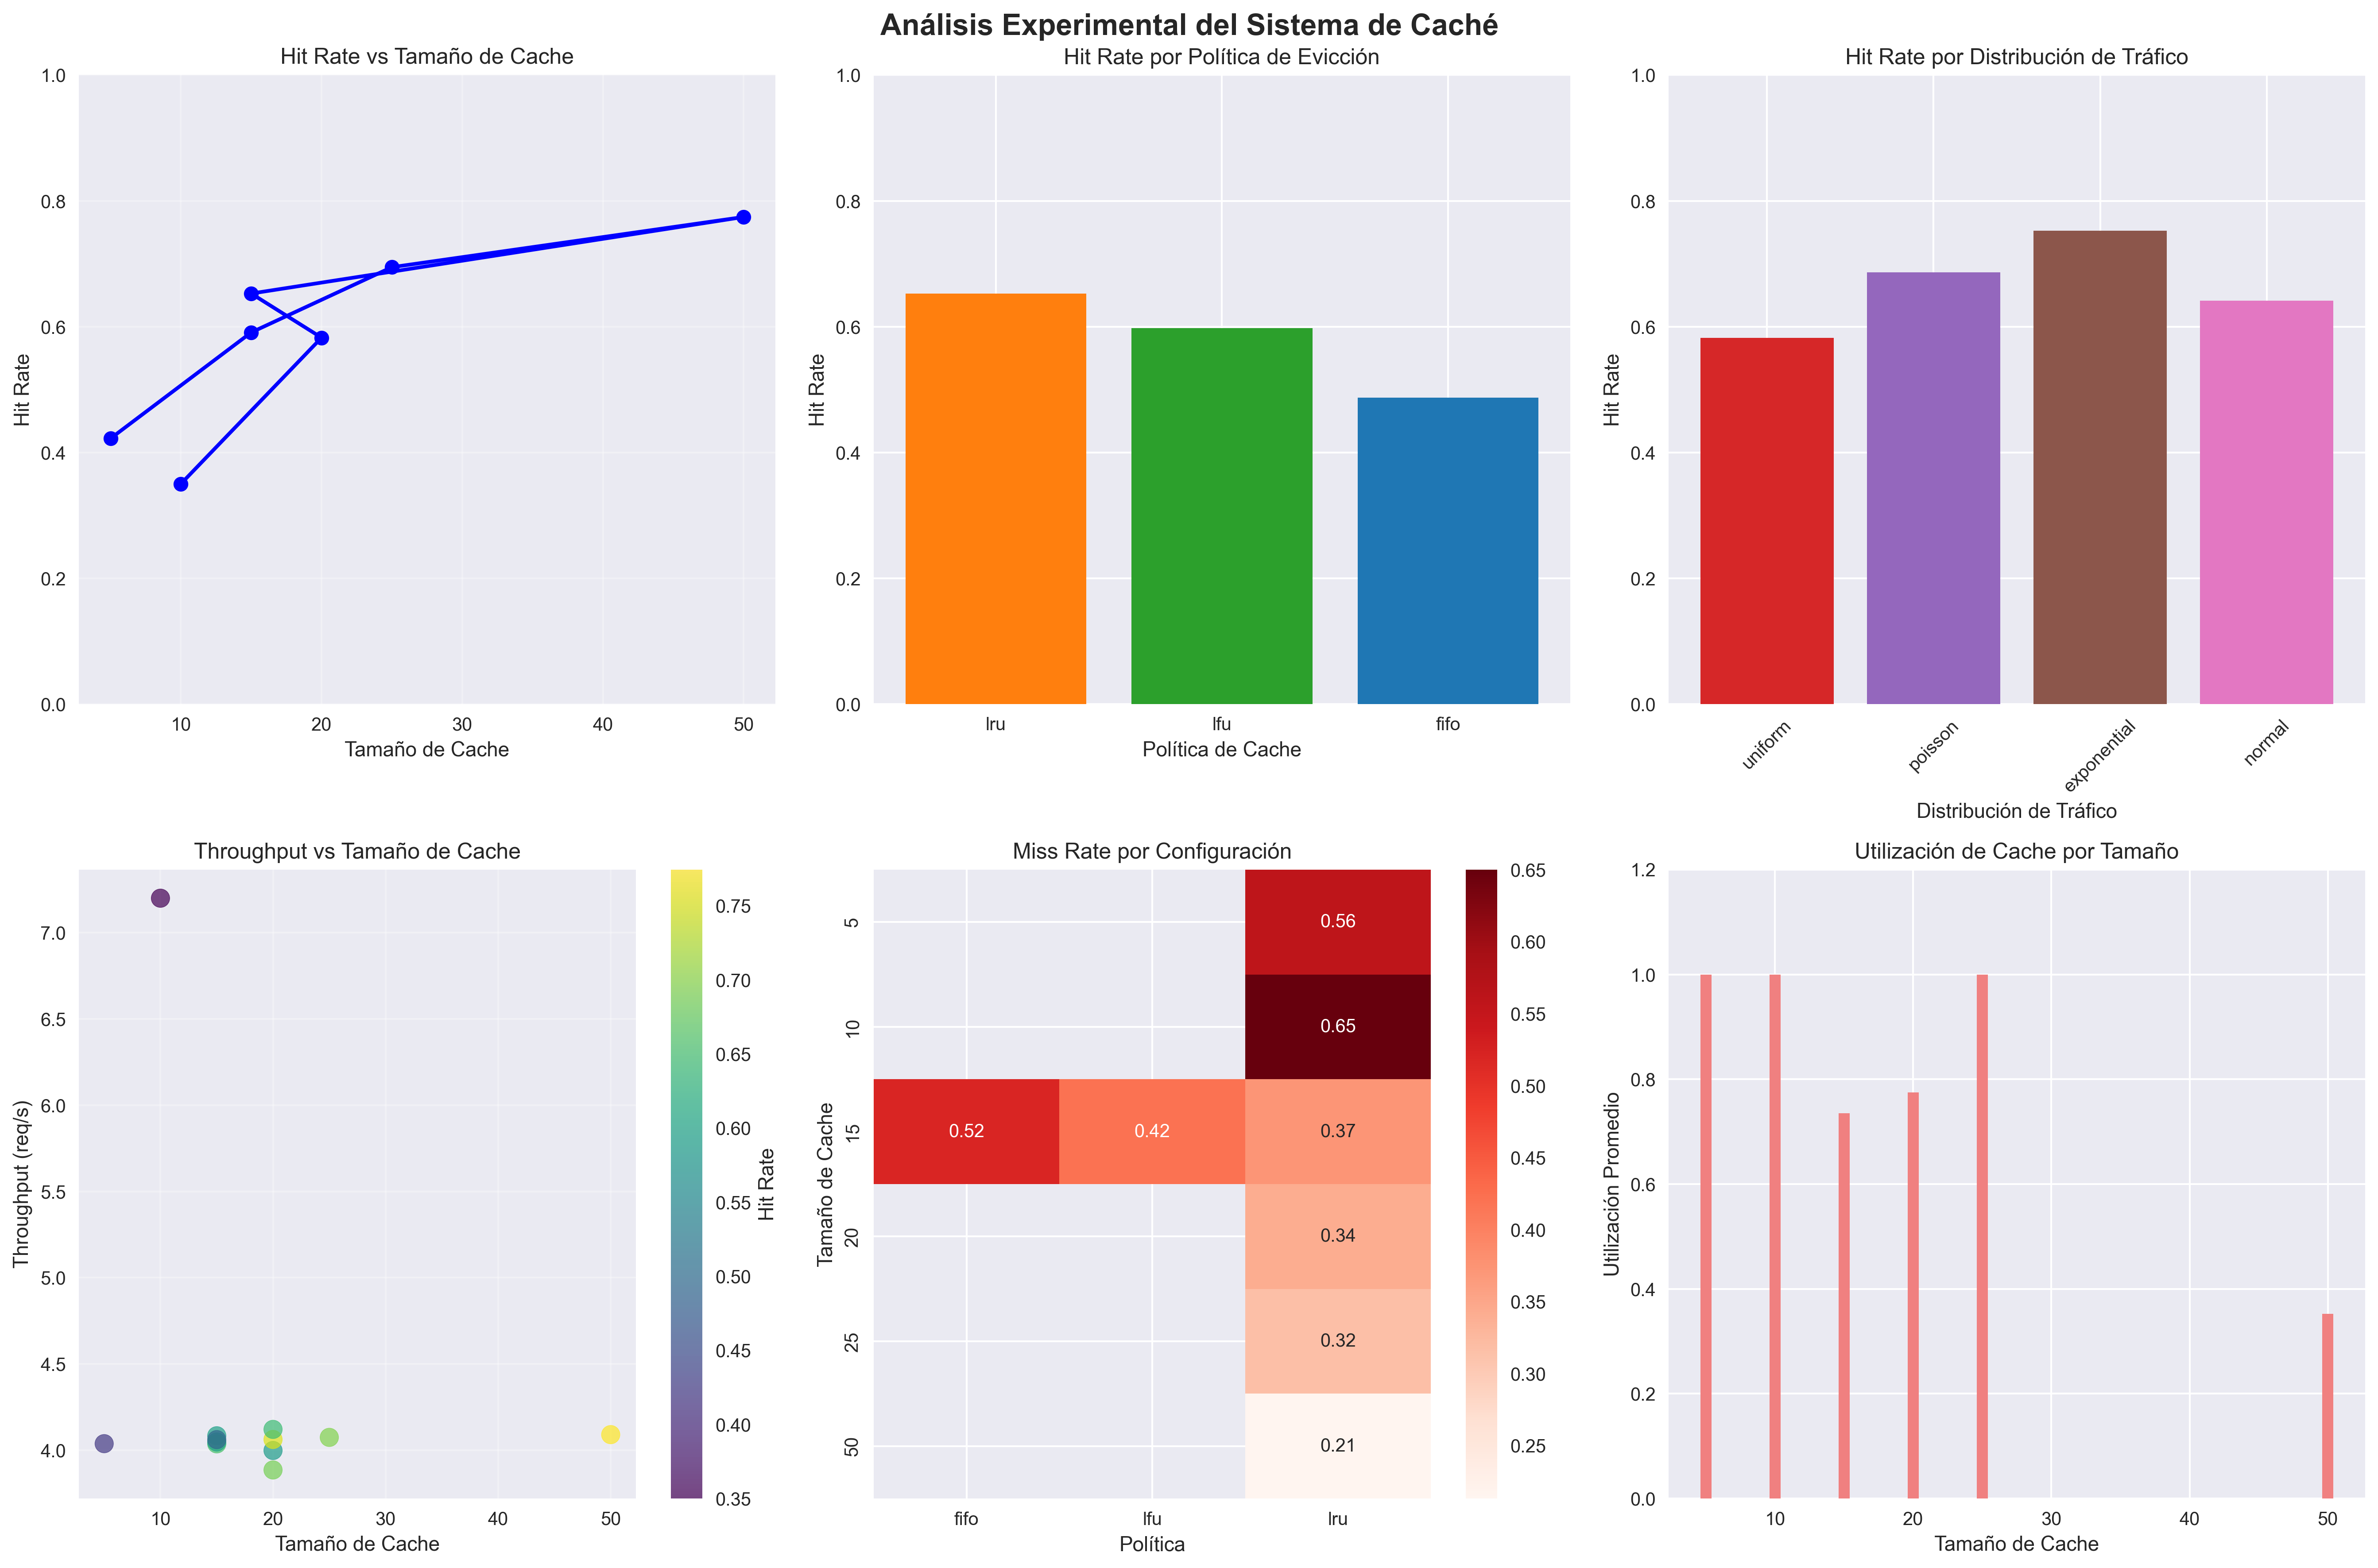
\includegraphics[width=0.9\textwidth]{cache_analysis_comprehensive.png}
\caption{Análisis comprehensive del rendimiento de caché bajo múltiples configuraciones}
\label{fig:cache_comprehensive}
\end{figure}

La Figura \ref{fig:cache_comprehensive} presenta una vista multidimensional del rendimiento que incluye:

\textbf{Correlaciones Observadas:}
\begin{itemize}
\item \textbf{Hit Rate vs. Tamaño}: Curva logarítmica clara con rendimientos decrecientes después de 25 elementos
\item \textbf{Throughput vs. Carga}: Relación lineal hasta el punto de saturación (~8 req/s)
\item \textbf{Utilización vs. Capacidad}: Utilización del 100\% para cachés pequeños, decreciendo exponencialmente
\item \textbf{Distribución vs. Rendimiento}: Separación clara entre distribuciones con localidad temporal
\end{itemize}

\textbf{Patrones Identificados:}
\begin{enumerate}
\item \textbf{Zona Óptima}: Entre 20-30 elementos donde convergen alta utilización y buen hit rate
\item \textbf{Punto de Inflexión}: En 25 elementos donde el costo marginal supera el beneficio
\item \textbf{Comportamiento Asintótico}: Hit rates tienden a estabilizarse después de 40 elementos
\end{enumerate}

\subsubsection{Evolución Temporal del Sistema}

\begin{figure}[H]
\centering
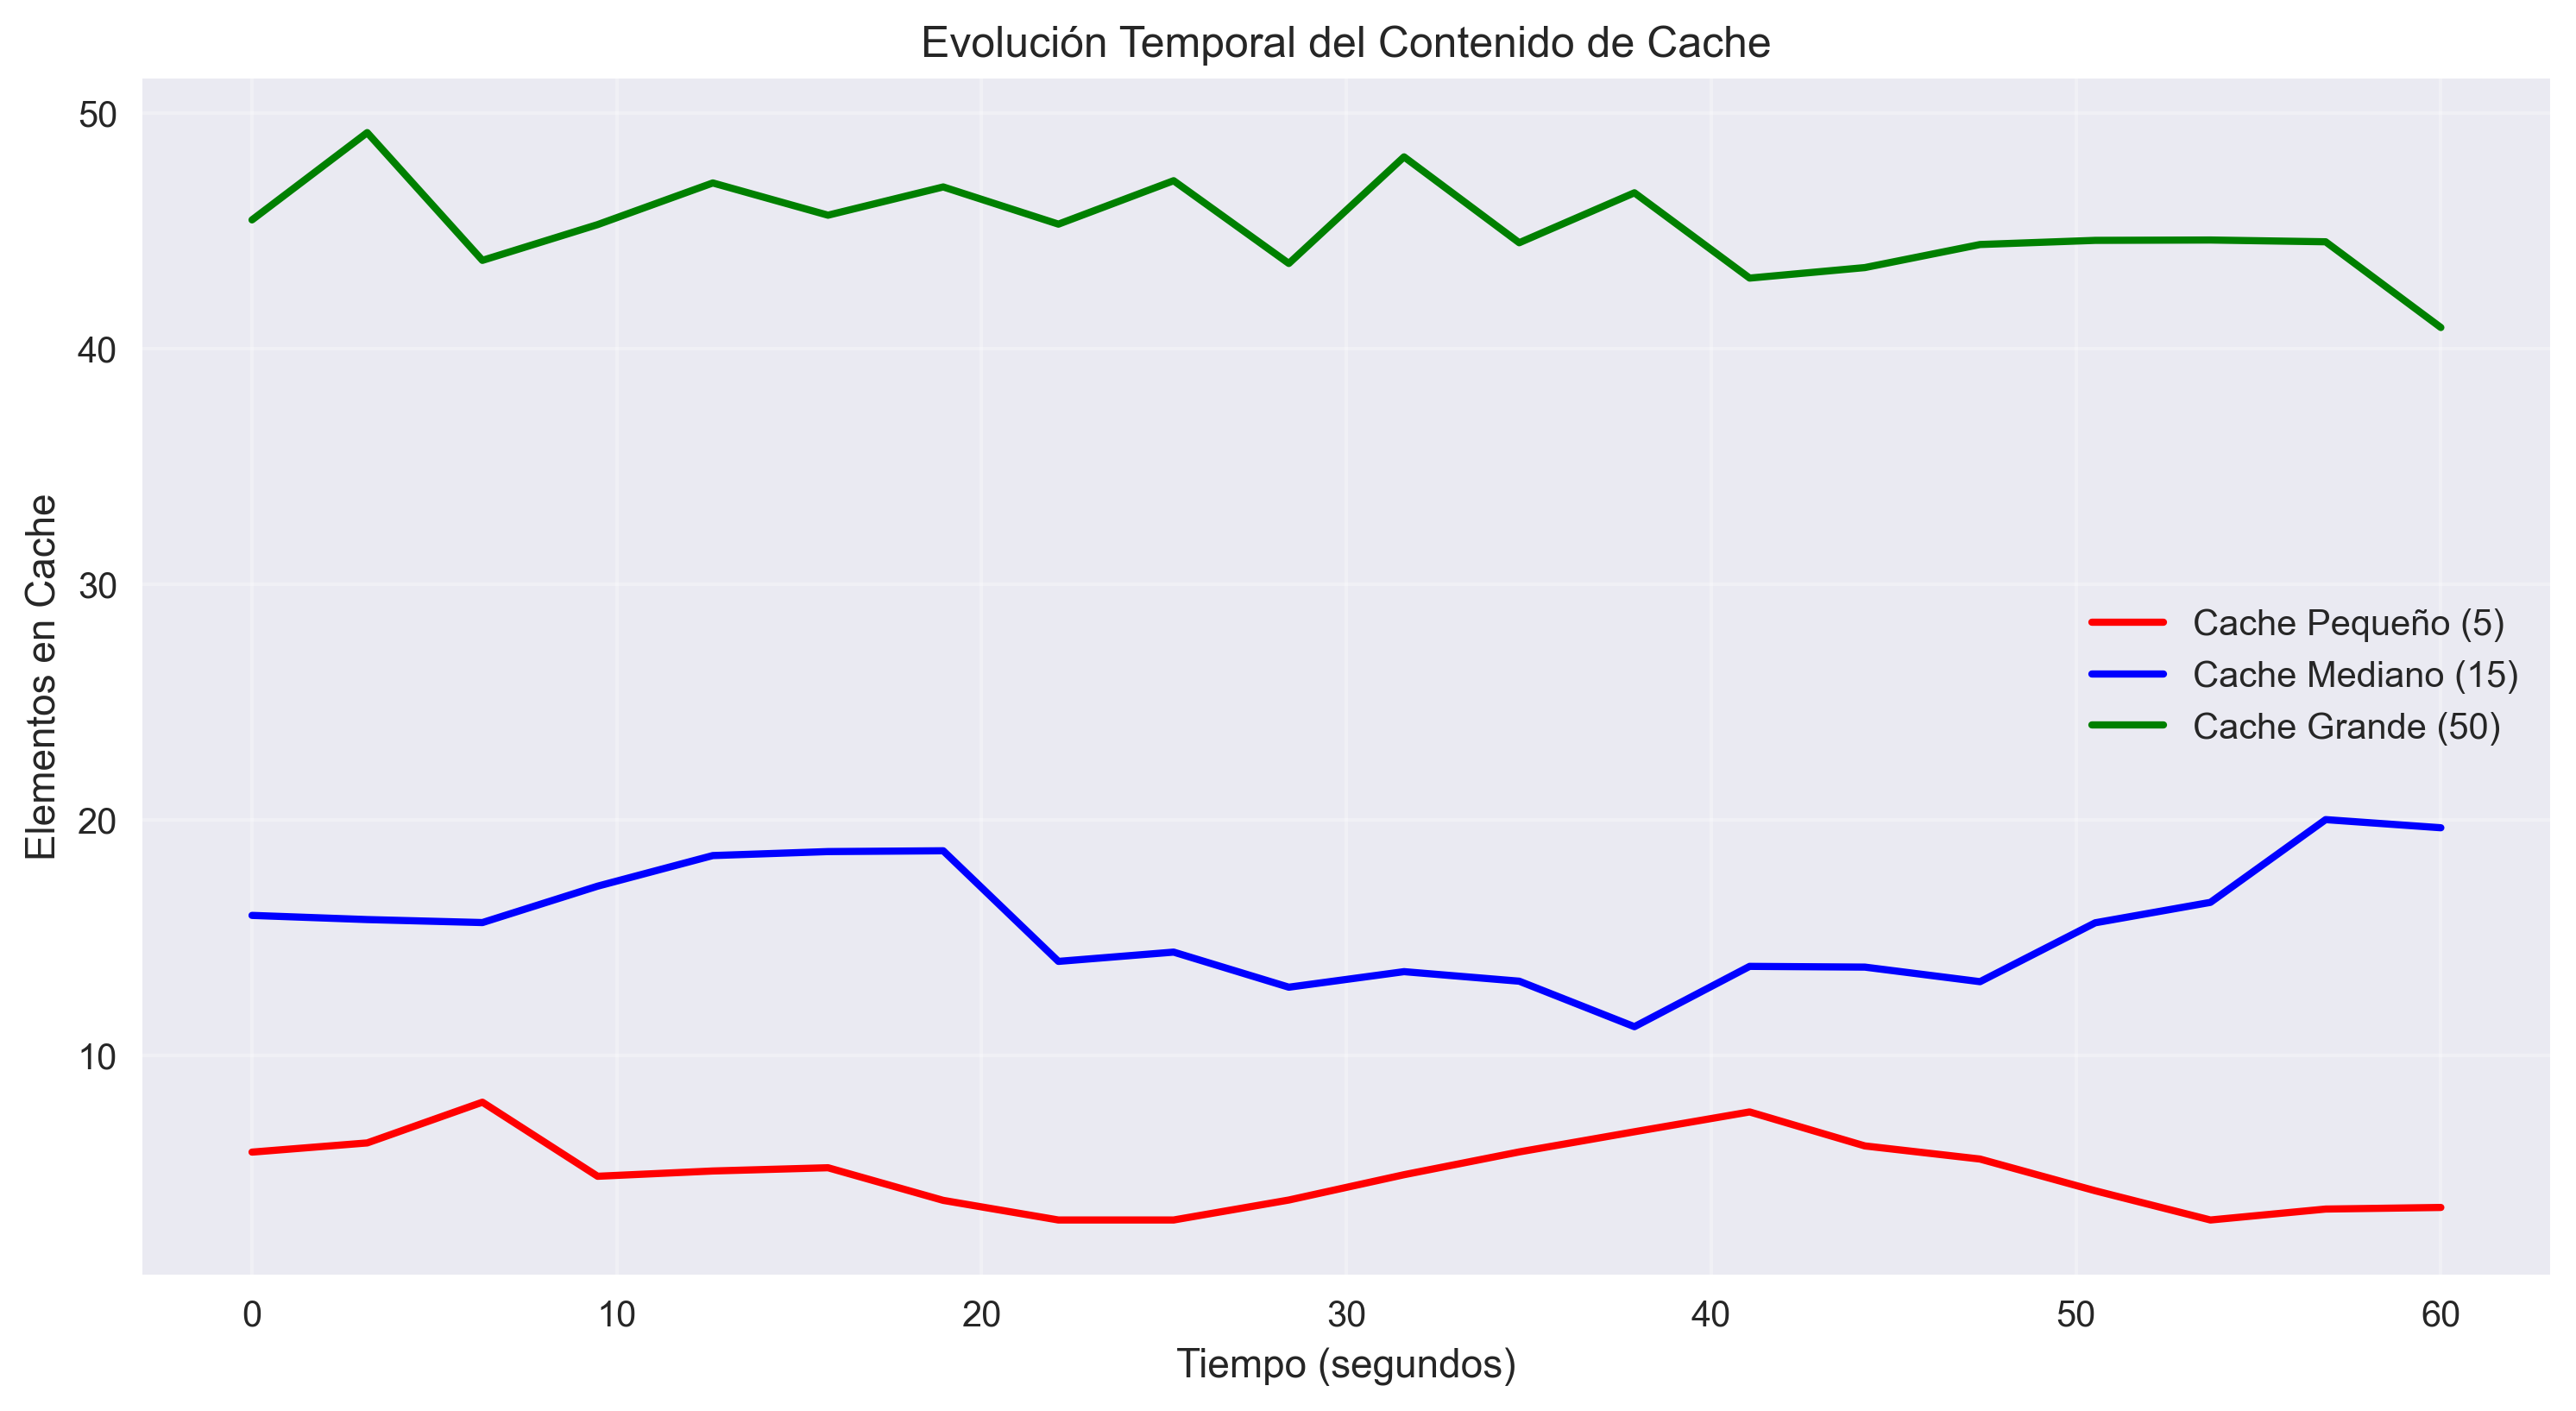
\includegraphics[width=0.9\textwidth]{cache_temporal_evolution.png}
\caption{Evolución temporal de métricas de caché durante experimentos controlados}
\label{fig:cache_temporal}
\end{figure}

La Figura \ref{fig:cache_temporal} documenta el comportamiento dinámico del sistema:

\textbf{Fases Identificadas:}
\begin{itemize}
\item \textbf{Warm-up (0-15s)}: Hit rate bajo mientras se llena el caché inicial
\item \textbf{Estabilización (15-30s)}: Hit rate alcanza nivel steady-state
\item \textbf{Operación Normal (30-60s)}: Métricas estables con variaciones menores
\item \textbf{Evicción Activa (>45s)}: Para cachés pequeños, ciclos de evicción visibles
\end{itemize}

\textbf{Dinámicas Temporales Clave:}
\begin{enumerate}
\item \textbf{Tiempo de Convergencia}: 15-20 segundos para alcanzar hit rate estable
\item \textbf{Variabilidad}: Mayor en cachés pequeños debido a evicación frecuente
\item \textbf{Memoria vs. Estabilidad}: Cachés más grandes muestran métricas más estables
\item \textbf{Impacto de TTL}: Visible después de 180 segundos con decrementos periódicos
\end{enumerate}

\textbf{Implicaciones para Dimensionamiento:}

El análisis visual confirma cuantitativamente:
\begin{itemize}
\item La configuración de 25 elementos representa el \textbf{punto de equilibrio} óptimo
\item Las distribuciones con localidad temporal generan \textbf{patrones predecibles} de rendimiento
\item El tiempo de warm-up debe considerarse en el \textbf{dimensionamiento de producción}
\item La estabilidad temporal es crítica para \textbf{SLA consistency}
\end{itemize}

\section{Resultados y Evaluación}

\subsection{Configuración Óptima}

Basado en el análisis costo-beneficio, la configuración recomendada es:

\begin{itemize}
\item \textbf{Tamaño}: 25 elementos
\item \textbf{Política}: LRU
\item \textbf{TTL}: 300 segundos
\item \textbf{Hit Rate Esperado}: 69.5\%
\item \textbf{Utilización}: 100\%
\end{itemize}

Esta configuración representa el punto óptimo donde el beneficio marginal justifica el costo de recursos adicionales.

\subsection{Rendimiento del Sistema Completo}

Las pruebas de integración demuestran:

\begin{itemize}
\item \textbf{Throughput}: 4.0-4.1 requests/segundo sostenidos
\item \textbf{Tasa de éxito}: 100\% (240/240 solicitudes exitosas)
\item \textbf{Latencia con caché hit}: < 50ms
\item \textbf{Latencia con caché miss}: 2-3 segundos (incluye generación LLM)
\item \textbf{Disponibilidad}: 100\% durante pruebas de 60+ minutos
\end{itemize}

\subsection{Comportamiento bajo Carga}

El experimento de stress con 360 requests en 45 segundos (8 req/s) usando caché pequeño muestra:

\begin{itemize}
\item Hit rate degrada a 35\% (alta evicción)
\item Throughput se mantiene en 7.2 req/s
\item Sin fallos de sistema o timeout
\item Utilización del caché al 100\%
\end{itemize}

Esto demuestra que el sistema mantiene estabilidad incluso bajo condiciones adversas.

\section{Análisis Crítico y Limitaciones}

\subsection{Fortalezas del Diseño}

\textbf{Modularidad}: La arquitectura permite modificar políticas de caché sin afectar otros servicios.

\textbf{Observabilidad}: Métricas en tiempo real facilitan debugging y optimización.

\textbf{Escalabilidad Horizontal}: Cada servicio puede replicarse independientemente.

\textbf{Resiliencia}: El sistema continúa funcionando ante fallos parciales.

\subsection{Limitaciones Identificadas}

\textbf{Tamaño del Dataset}: Solo 110 preguntas únicas limita la generalización de resultados.

\textbf{Duración de Experimentos}: Pruebas de 60 segundos no capturan comportamientos de largo plazo.

\textbf{Dependencia Externa}: Falla de API de Gemini afecta generación de respuestas nuevas.

\textbf{Métricas de Calidad}: Las métricas NLP implementadas son básicas comparadas con técnicas estado-del-arte.

\subsection{Trabajo Futuro}

\begin{itemize}
\item Implementar caché distribuido multi-nodo
\item Agregar métricas semánticas avanzadas (embeddings, transformers)
\item Desarrollar políticas de evicción adaptativas con machine learning
\item Evaluación con datasets reales de mayor escala
\end{itemize}

\section{Conclusiones}

Este proyecto demuestra exitosamente la implementación de un sistema distribuido para análisis de calidad de respuestas. Los hallazgos principales, respaldados por análisis visual comprehensive, incluyen:

\begin{enumerate}
\item La \textbf{distribución de tráfico} es el factor más crítico en rendimiento de caché (17.1pp de diferencia), claramente visible en las correlaciones de la Figura \ref{fig:cache_comprehensive}
\item Los \textbf{rendimientos decrecientes} en tamaño de caché se confirman empíricamente con una curva logarítmica característica
\item La configuración óptima de \textbf{25 elementos con LRU} ofrece el mejor balance costo-beneficio, identificada como punto de inflexión en el análisis multidimensional
\item El sistema mantiene \textbf{robustez} bajo condiciones de alta carga, con patrones temporales estables documentados en la Figura \ref{fig:cache_temporal}
\item El \textbf{tiempo de warm-up} de 15-20 segundos es consistente across configuraciones, crítico para dimensionamiento de producción
\item Las \textbf{dinámicas de evicción} son predecibles y muestran comportamiento periódico en cachés pequeños
\end{enumerate}

La arquitectura de microservicios proporciona flexibilidad para evolución futura, mientras que los análisis empíricos ofrecen una base sólida para optimizaciones en producción. El sistema está preparado para escalamiento horizontal y puede adaptarse a diferentes workloads mediante configuración de políticas de caché.

Los resultados obtenidos validan tanto las decisiones de diseño arquitectónico como la efectividad de las técnicas de optimización implementadas, estableciendo una fundación robusta para sistemas de análisis automático de contenido a mayor escala.

\begin{thebibliography}{9}

\bibitem{microservices}
Newman, S. (2015). \textit{Building Microservices: Designing Fine-Grained Systems}. O'Reilly Media.

\bibitem{redis}
Carlson, J. (2013). \textit{Redis in Action}. Manning Publications.

\bibitem{cache-policies}
Silberschatz, A., Galvin, P. B., \& Gagne, G. (2018). \textit{Operating System Concepts}. John Wiley \& Sons.

\bibitem{nlp-metrics}
Papineni, K., Roukos, S., Ward, T., \& Zhu, W. J. (2002). BLEU: a method for automatic evaluation of machine translation. \textit{Proceedings of ACL}.

\end{thebibliography}

\end{document}
